\documentclass{article}

% Language setting
% Replace `english' with e.g. `spanish' to change the document language
\usepackage[english]{babel}

% Set page size and margins
% Replace `letterpaper' with `a4paper' for UK/EU standard size
\usepackage[letterpaper,top=2cm,bottom=2cm,left=3cm,right=3cm,marginparwidth=1.75cm]{geometry}

% Useful packages
\usepackage{amsmath}
\usepackage{graphicx}
\usepackage[colorlinks=true, allcolors=blue]{hyperref}


\begin{document}



\section{Channel selection}

Channel selection is one of the possible solutions when it comes to reducing the amount of data we send from one transmitter to the other.
Our objective is clearly to send as much informative data as possible, but that comes with a cost that we may not be able to deal with, depending on other critical points we have seen.
Moreover not all signals carry useful information, some of them may just add noise and complicate our classification of neural data.
Because of this, channel selection is not just a feat of data size optimization but of accuracy optimization as well.
By removing noise we can increment our accuracy and by removing less informative channels we can send data effectively without having to worry about the critical point we have previously stated.

\subsection{Signal data}

Here I describe the structure of data, saying the rationale behind the cuff electrode signals.
Why radial and longitudinal etc...
We cut to 10 channels more or less so we send the signal and we can handle that data size.
The problem with the data is that since we apply electrode cuffs chirurgically there may be noise added and electrodes that straight up work poorly.
Therefore we need to define a precise pipeline that can discard non informative signal or worse, noise from our channels.
Ideally, if we would discard more than 16 channels and have less than 10, we could try to perform some sort of de-noise over the channels.


\begin{figure}[h]
      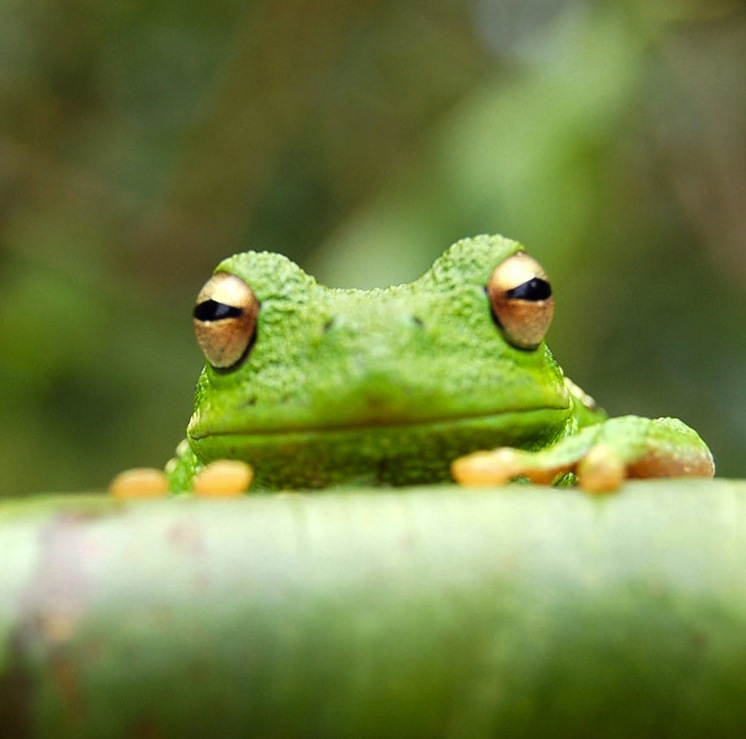
\includegraphics[width=8cm]{Images/frog.jpg}
\end{figure}





\subsection{Requirements and Specifications}

We have a setup time that includes many procedures.
So we do not have a lot of time for training and processing.
We receive our data in two different streams.
A first stream composed of 8 channels that lasts 1 minute.
A second stream with the remaining 8 channels that lasts again 1 minute.
Also our setup is composed of small micro-controllers that can perform little to no calculation.
We have to keep in mind a few things.
\begin{itemize}
\item We cannot train after having received the data cause it would take too much time
\item We cannot train beforehand a specific model since the data we have is different from the one we will receive.
\item Possibility is to train a very general auto encoder that can compress data and add some sort of de-noise by removing the wrong information.
\item and like this.
\end{itemize}

However, there is a problem in the previous studies. The effect of the same algorithm on different subjects is quite different. Research on reducing the impact of differences between individuals on the classification performance is the core work of this paper.
{DWT and CNN based multi-class motor imagery electroencephalographic signal recognition}

Because of these restrictions the best methodology is an online approach that can evaluate the channels either while we are receiving them or right after the transmission is over.
Cross-Correlation Based Discriminant Criterion emerges as the best solution [Cross-Correlation Based Discriminant Criterion for
Channel Selection in Motor Imagery BCI Systems], especially when paired with a CNN classifier such as the ENGNet we implemented based on [] as shown in this review at 1.2.[https://www.ncbi.nlm.nih.gov/pmc/articles/PMC9774545/]


\subsection{Pipeline of the work}
@zhangMotorImageryRecognition2021

\begin{itemize}
\item Read data
\item Analyze by metrics that depend only on the signal itself (variance etc...) if we can
\item ASR 
\item Cross-correlate within channels
\item CNN
\item Pack the signal and send i
\end{itemize}


\subsection{Cross-correlation and evidence}
{Wavelet Coherence Based Channel Selection for Classifying Single Trial Motor Imagery}
{Cross-Correlation Based Discriminant Criterion for
Channel Selection in Motor Imagery BCI Systems}
XCDC measures similarity between signals by
cross-correlation, and emphasizes the electrodes that:
1) signals of the same class show larger similarity, and
2) signals of different classes differ more obviously.
After ranking the channels according to XCDC, signals
from the channels with highest discriminant criterion
are chosen as the input of a convolutional neural
network (CNN) classifier, which further evaluates the
credibility of the chosen channels by classification
accuracy. The performance of XCDC is evaluated
and compared to CCS [26] and CSP-rank and is better than both (change this).
The complexity of XCDC is quadratic. Deriving
the discriminant score D of a channel involves the
computation of cross-correlation between every pair of
trials, resulting in a quadratic complexity.


\subsection{Artifact subspace reconstruction (ASR)}
Artifact subspace reconstruction (ASR) is an automatic, online-capable, component-based method that can effectively remove transient or large-amplitude artifacts contaminating electroencephalographic (EEG) data
{Evaluation of Artifact Subspace Reconstruction for Automatic Artifact Components Removal in Multi-Channel EEG Recordings}


\subsection{Genetic Algorithm why not (BPSO) and why not in general wrapper methods}
{Filtering techniques for channel selection in motor imagery EEG applications: a survey}
{A review of channel selection algorithms for EEG signal processing}
{EEG electrode selection method based on BPSO with channel impact factor for acquisition of significant brain signal}

\subsection{Evaluation of channel selection methods by building a classifier (CNN)}

Why EEGNet...

\subsection{Overall staple}
{EEG Channel Selection Techniques in Motor Imagery Applications: A Review and New Perspectives}























\section{Some examples to get started}

\subsection{How to create Sections and Subsections}

Simply use the section and subsection commands, as in this example document! With Overleaf, all the formatting and numbering is handled automatically according to the template you've chosen. If you're using the Visual Editor, you can also create new section and subsections via the buttons in the editor toolbar.

\subsection{How to include Figures}

First you have to upload the image file from your computer using the upload link in the file-tree menu. Then use the includegraphics command to include it in your document. Use the figure environment and the caption command to add a number and a caption to your figure. See the code for Figure \ref{fig:frog} in this section for an example.

Note that your figure will automatically be placed in the most appropriate place for it, given the surrounding text and taking into account other figures or tables that may be close by. You can find out more about adding images to your documents in this help article on \href{https://www.overleaf.com/learn/how-to/Including_images_on_Overleaf}{including images on Overleaf}.


\subsection{How to add Tables}

Use the table and tabular environments for basic tables --- see Table~\ref{tab:widgets}, for example. For more information, please see this help article on \href{https://www.overleaf.com/learn/latex/tables}{tables}. 



\subsection{How to add Comments and Track Changes}

Comments can be added to your project by highlighting some text and clicking ``Add comment'' in the top right of the editor pane. To view existing comments, click on the Review menu in the toolbar above. To reply to a comment, click on the Reply button in the lower right corner of the comment. You can close the Review pane by clicking its name on the toolbar when you're done reviewing for the time being.

Track changes are available on all our \href{https://www.overleaf.com/user/subscription/plans}{premium plans}, and can be toggled on or off using the option at the top of the Review pane. Track changes allow you to keep track of every change made to the document, along with the person making the change. 

\subsection{How to add Lists}

You can make lists with automatic numbering \dots

\begin{enumerate}
\item Like this,
\item and like this.
\end{enumerate}
\dots or bullet points \dots
\begin{itemize}
\item Like this,
\item and like this.
\end{itemize}

\subsection{How to write Mathematics}

\LaTeX{} is great at typesetting mathematics. Let $X_1, X_2, \ldots, X_n$ be a sequence of independent and identically distributed random variables with $\text{E}[X_i] = \mu$ and $\text{Var}[X_i] = \sigma^2 < \infty$, and let
\[S_n = \frac{X_1 + X_2 + \cdots + X_n}{n}
      = \frac{1}{n}\sum_{i}^{n} X_i\]
denote their mean. Then as $n$ approaches infinity, the random variables $\sqrt{n}(S_n - \mu)$ converge in distribution to a normal $\mathcal{N}(0, \sigma^2)$.


\subsection{How to change the margins and paper size}

Usually the template you're using will have the page margins and paper size set correctly for that use-case. For example, if you're using a journal article template provided by the journal publisher, that template will be formatted according to their requirements. In these cases, it's best not to alter the margins directly.

If however you're using a more general template, such as this one, and would like to alter the margins, a common way to do so is via the geometry package. You can find the geometry package loaded in the preamble at the top of this example file, and if you'd like to learn more about how to adjust the settings, please visit this help article on \href{https://www.overleaf.com/learn/latex/page_size_and_margins}{page size and margins}.

\subsection{How to change the document language and spell check settings}

Overleaf supports many different languages, including multiple different languages within one document. 

To configure the document language, simply edit the option provided to the babel package in the preamble at the top of this example project. To learn more about the different options, please visit this help article on \href{https://www.overleaf.com/learn/latex/International_language_support}{international language support}.

To change the spell check language, simply open the Overleaf menu at the top left of the editor window, scroll down to the spell check setting, and adjust accordingly.

\subsection{How to add Citations and a References List}

You can simply upload a \verb|.bib| file containing your BibTeX entries, created with a tool such as JabRef. You can then cite entries from it, like this: \cite{greenwade93}. Just remember to specify a bibliography style, as well as the filename of the \verb|.bib|. You can find a \href{https://www.overleaf.com/help/97-how-to-include-a-bibliography-using-bibtex}{video tutorial here} to learn more about BibTeX.

If you have an \href{https://www.overleaf.com/user/subscription/plans}{upgraded account}, you can also import your Mendeley or Zotero library directly as a \verb|.bib| file, via the upload menu in the file-tree.

\subsection{Good luck!}

We hope you find Overleaf useful, and do take a look at our \href{https://www.overleaf.com/learn}{help library} for more tutorials and user guides! Please also let us know if you have any feedback using the Contact Us link at the bottom of the Overleaf menu --- or use the contact form at \url{https://www.overleaf.com/contact}.

\bibliographystyle{alpha}
\bibliography{sample}

\end{document}